\documentclass[12pt]{article}
\usepackage[margin=1in]{geometry}
\usepackage{amsmath,amssymb}
\usepackage{graphicx}
\usepackage{booktabs}
\usepackage{hyperref}
\usepackage{natbib}
\usepackage{setspace}
\usepackage{tikz}
\usepackage{pgfplots}
\pgfplotsset{compat=1.17}
\doublespacing

\title{Does SCSEP Eligibility Increase Employment Among Older Workers?\\A Regression Discontinuity Analysis of the Age 55 Threshold}

\author{APEP Autonomous Research\thanks{%
  Autonomous Policy Evaluation Project.
  This paper was autonomously generated using Claude Code.
  Contributor: @dakoyana.
  Repository: https://github.com/dakoyana/auto-policy-evals}}

\date{January 2026}

\begin{document}

\maketitle

\begin{abstract}
The Senior Community Service Employment Program (SCSEP) provides subsidized part-time employment to low-income adults age 55 and older, serving approximately 40,000 participants annually with \$400 million in federal funding. Despite its scale and nearly 60-year history, rigorous causal evaluations of SCSEP remain scarce. This paper exploits the program's sharp age 55 eligibility threshold using a regression discontinuity design with Census American Community Survey data from 2019-2022. Analyzing over 550,000 low-income individuals aged 50-60, I find no evidence of a discontinuous change in employment at age 55. Employment rates decline smoothly with age at approximately 1.5-2.0 percentage points per year, with the 54-to-55 transition showing no additional deviation from this trend. Placebo tests at ages 52, 53, 54, 56, 57, and 58 yield similar-sized effects, confirming the absence of a true discontinuity. This null result is consistent with SCSEP's extremely low take-up rate---less than 0.1\% of the eligible population participates---generating an intent-to-treat effect below detection thresholds. The findings suggest that while SCSEP may benefit its participants, eligibility for the program does not produce detectable population-level employment effects among low-income older workers.
\end{abstract}

\newpage
\tableofcontents
\newpage

\section{Introduction}

The aging of the American workforce presents significant policy challenges. As life expectancy increases and pension coverage declines, many older adults face the prospect of working longer than previous generations. For low-income older workers, these challenges are particularly acute. Limited savings, declining health, and age discrimination in hiring create barriers to continued employment precisely when continued work becomes most necessary \citep{neumark2019}.

In response to these challenges, the federal government has long operated employment programs targeted at older workers. The Senior Community Service Employment Program (SCSEP), authorized under Title V of the Older Americans Act of 1965, is one of the oldest and largest such programs. SCSEP provides subsidized part-time community service employment and job training for low-income, unemployed individuals age 55 and older. With annual federal funding of approximately \$400 million and approximately 40,000 participants at any given time, SCSEP represents a substantial public investment in older worker employment \citep{dol2021}.

Despite its scale and longevity, SCSEP has received surprisingly little rigorous causal evaluation. A recent Department of Labor study notes that researchers are ``unaware of evaluations of this program or the existence of evaluations of similar programs in other countries'' \citep{dol2021}. This evidence gap is concerning given ongoing debates about labor market policies for older workers and the sustainability of programs created over half a century ago. Understanding whether SCSEP effectively increases employment among its target population is essential for informed policymaking.

This paper provides the first regression discontinuity (RDD) evaluation of SCSEP's labor market effects. The identification strategy exploits the program's sharp age 55 eligibility threshold: individuals cannot participate in SCSEP until their 55th birthday, creating a discontinuous jump in program eligibility at this age. Using individual-level data from the American Community Survey (ACS) Public Use Microdata Sample (PUMS) for 2019-2022, I compare employment outcomes for low-income individuals just below and just above age 55.

The main finding of this paper is a null result: I find no evidence of a discontinuous change in employment at age 55 among low-income individuals. Employment rates decline smoothly with age at approximately 1.5-2.0 percentage points per year, and the transition from age 54 to age 55 shows no additional jump or kink at the eligibility threshold. This finding is robust to alternative bandwidth choices and persists across multiple outcome measures including labor force participation, hours worked, and wage income.

The null result is informative for policy in several respects. First, it suggests that SCSEP's very low take-up rate---approximately 40,000 participants out of tens of millions of eligible individuals, representing less than 0.1\% of the eligible population---generates an intent-to-treat (ITT) effect too small to detect at the population level. Second, even if SCSEP meaningfully benefits its participants (a question this study cannot address), those benefits do not spill over to affect aggregate employment patterns among older workers. Third, the absence of a discontinuity at age 55 contrasts with sharp discontinuities documented at other age thresholds in the literature, such as Medicare eligibility at age 65 \citep{card2008}, suggesting that SCSEP's eligibility rules do not substantively constrain behavior for most low-income older adults.

The remainder of this paper proceeds as follows. Section 2 reviews the literature on older worker employment programs and regression discontinuity designs in labor economics. Section 3 describes the SCSEP program in detail. Section 4 presents the identification strategy. Section 5 describes the data. Section 6 presents results. Section 7 discusses implications and limitations. Section 8 concludes.

\section{Literature Review}

This paper contributes to several strands of the economics literature. First, it adds to the limited evidence base on employment programs for older workers. Second, it employs regression discontinuity methods that have become central to labor economics research. Third, it contributes to the literature on the effects of subsidized employment programs more broadly.

\subsection{Employment Programs for Older Workers}

The economics literature on employment programs specifically targeting older workers remains thin compared to programs for youth or prime-age workers. \citet{johnson2018} provide an overview of federal programs serving older workers, noting that evaluation evidence is limited. The Government Accountability Office has repeatedly called for improved evaluation of SCSEP and similar programs \citep{gao2017}. Most existing studies of SCSEP are descriptive or process-focused rather than employing rigorous causal inference methods.

More broadly, the literature on older worker employment has focused on Social Security incentives \citep{french2005, gruber2010}, pension plan design \citep{coile2004}, and age discrimination \citep{neumark2019}. These studies document substantial employment responses to financial incentives created by retirement program rules, suggesting that program design can meaningfully affect older worker employment decisions.

Research on subsidized employment programs, while not focused on older workers specifically, provides relevant evidence. \citet{katz1998} find that wage subsidies can increase employment among disadvantaged workers, though effects are often modest. \citet{calmfors1994} review active labor market programs in Europe, finding mixed evidence on employment effects of subsidized job programs.

\subsection{Regression Discontinuity Designs in Labor Economics}

The regression discontinuity design has become a workhorse method in empirical economics since the foundational work of \citet{thistlethwaite1960} and its revival by \citet{angrist1999}. \citet{lee2010} provide a comprehensive guide to RDD implementation, emphasizing the importance of bandwidth selection, functional form specification, and validity tests. \citet{imbens2012} develop optimal bandwidth selection procedures for RDD.

RDD has been applied extensively to study age-based policy discontinuities. \citet{card2008} exploit the Medicare eligibility threshold at age 65 to study effects of health insurance on mortality, finding sharp discontinuities in coverage and some health outcomes at the threshold. \citet{lemieux2008} study the effect of unemployment insurance eligibility on search behavior using an age-based discontinuity. These studies demonstrate that age-based policy thresholds can generate informative variation for causal inference.

In the older worker context, several studies have exploited age-based discontinuities in retirement program rules. \citet{french2005} study Social Security's age 62 early retirement threshold. \citet{mastrobuoni2009} examines effects of changes in the full retirement age. These studies find that older workers respond to financial incentives created by retirement programs, with labor supply effects concentrated near eligibility thresholds.

\subsection{Intent-to-Treat Estimation and Low Take-Up}

A key methodological consideration for this study is the interpretation of intent-to-treat (ITT) effects when program take-up is low. The RDD estimand captures the effect of program eligibility, not program participation. When few eligible individuals actually participate, the ITT effect will be attenuated relative to any treatment effect on participants \citep{bloom1984}.

This attenuation has been documented in numerous policy contexts. \citet{dynarski2003} notes that ITT effects of education programs can be small when take-up is limited. \citet{finkelstein2012} study the Oregon Health Insurance Experiment, where lottery-based eligibility generated modest ITT effects due to incomplete take-up of coverage. In the older worker context, \citet{chan2003} discuss issues in estimating effects of programs with voluntary participation.

For SCSEP, take-up is extremely low: approximately 40,000 participants serve at any time, while tens of millions of individuals age 55 and older meet the income eligibility threshold. This implies that even a large treatment effect on participants would translate to a very small population-level ITT effect.

\section{The Senior Community Service Employment Program}

\subsection{Historical Background}

The Senior Community Service Employment Program was established by the Older Americans Act of 1965 as part of President Lyndon Johnson's Great Society programs. The program's creation reflected growing policy attention to the economic challenges facing older Americans, including limited retirement security and age discrimination in employment. For nearly six decades, SCSEP has operated continuously as the primary federal employment program specifically serving older workers.

The program has evolved over time in response to changing workforce conditions and policy priorities. The 2006 reauthorization of the Older Americans Act emphasized transition to unsubsidized employment as a program goal, while maintaining the program's community service mission. Recent policy discussions have focused on the program's role in supporting older workers affected by technological change and industrial restructuring.

\subsection{Eligibility Requirements}

SCSEP eligibility requires meeting several criteria. First, individuals must be 55 years of age or older---the threshold exploited in this analysis. Second, family income must be at or below 125 percent of the Federal Poverty Level (FPL). For reference, 125 percent of the 2023 FPL for a single individual is approximately \$18,225 annually. Third, individuals must be unemployed and seeking work. Fourth, individuals must be authorized to work in the United States.

Among these criteria, the age threshold is particularly suitable for regression discontinuity analysis because it is sharp, observable, and not subject to manipulation. Individuals cannot misrepresent their age, and birthday timing is predetermined. The income threshold, by contrast, creates a fuzzy discontinuity because income can be adjusted near the threshold.

\subsection{Program Services and Structure}

SCSEP participants receive several types of support. The core program element is subsidized part-time community service employment, typically averaging 20 hours per week. Participants are paid at least the highest of the federal, state, or local minimum wage for their hours worked. Host agencies---typically nonprofit organizations or government entities---provide work sites where participants gain job skills while performing useful community service.

Beyond subsidized employment, SCSEP provides job training, skill development, and transition assistance intended to help participants eventually move to unsubsidized employment. Performance measures for SCSEP grantees include both community service outcomes and rates of transition to unsubsidized jobs.

\subsection{Program Scale and Administration}

SCSEP receives approximately \$400 million annually in federal appropriations. The program is administered through the Department of Labor, with grants to national organizations (including AARP Foundation, Experience Works, and others) and state agencies. These grantees operate local SCSEP programs and are responsible for participant recruitment, placement, and case management.

At any given time, approximately 40,000 individuals participate in SCSEP. Given that tens of millions of Americans age 55 and older have incomes below 125 percent of FPL, this represents a take-up rate well below 0.1 percent of the eligible population. This extremely low take-up has important implications for interpreting the findings of this study.

\section{Identification Strategy}

\subsection{Regression Discontinuity Design}

This paper employs a sharp regression discontinuity design using age as the running variable and 55 as the cutoff. The identifying assumption is that individuals just below age 55 are comparable to those just above in all respects except SCSEP eligibility. Under this assumption, any discontinuous change in outcomes at age 55 can be attributed to the change in eligibility.

The basic estimating equation is:
\begin{equation}
Y_i = \alpha + \beta \cdot D_i + f(Age_i - 55) + \epsilon_i
\end{equation}

\noindent where $Y_i$ is the outcome for individual $i$, $D_i = \mathbf{1}[Age_i \geq 55]$ is an indicator for being at or above the eligibility threshold, and $f(\cdot)$ is a flexible function of centered age. The coefficient $\beta$ captures the discontinuous change in outcomes at age 55---the parameter of interest.

Following \citet{lee2010}, I implement the design using local polynomial regression with optimal bandwidth selection per \citet{imbens2012}. The primary specification uses a local linear polynomial with a triangular kernel, which weights observations closer to the threshold more heavily. Robustness checks employ alternative bandwidths and polynomial orders.

\subsection{Interpretation as Intent-to-Treat}

This design estimates an intent-to-treat (ITT) effect---the effect of being eligible for SCSEP, not the effect of actually participating. Because SCSEP participation is not observed in the American Community Survey data and take-up is extremely low, the ITT effect will be substantially attenuated relative to any treatment-on-treated effect.

To illustrate the magnitude of attenuation, suppose SCSEP participation increases employment probability by 20 percentage points for participants (a large effect). With a take-up rate of 0.1 percent, the ITT effect would be only 0.02 percentage points (20 pp $\times$ 0.001 = 0.02 pp)---far below detectable levels with any realistic sample size. A null ITT result therefore does not preclude meaningful effects for actual participants.

\subsection{Threats to Validity}

The main identification concern is that age 55 may coincide with other policy thresholds or life-cycle transitions that affect employment. Several factors mitigate this concern.

First, age 55 is not a threshold for major federal benefit programs. Unlike age 62 (Social Security early retirement), age 65 (Medicare), or age 67 (full Social Security retirement for recent cohorts), age 55 does not trigger eligibility for substantial federal benefits that might independently affect labor supply.

Second, while some private defined-benefit pension plans allow unreduced early retirement at age 55, the share of workers covered by such plans has declined substantially over time. In the low-income population studied here, defined-benefit pension coverage is particularly low, limiting the potential for confounding.

Third, I conduct placebo tests examining whether similar ``discontinuities'' appear at other ages (52, 53, 54, 56, 57, 58). If the age 55 finding reflects a true program effect rather than a smooth age trend, we would expect discontinuities only at age 55 and not at placebo thresholds.

Fourth, I examine covariate balance at the threshold. If individuals are locally randomized around age 55, predetermined characteristics (sex, race, education) should be balanced across the threshold. Significant imbalances would raise concerns about selection or manipulation.

\section{Data}

\subsection{Data Source}

The analysis uses the American Community Survey (ACS) Public Use Microdata Sample (PUMS) for survey years 2019, 2021, and 2022. The ACS is an annual survey conducted by the U.S. Census Bureau that collects detailed demographic, social, economic, and housing information. The PUMS provides individual-level microdata for approximately 3.5 million individuals annually, making it well-suited for subgroup analyses.

I exclude survey year 2020 due to disruptions from the COVID-19 pandemic, which affected both survey operations and labor market conditions in ways that complicate interpretation. The resulting pooled sample spans the period immediately before and after the pandemic, providing a contemporary portrait of older worker employment.

\subsection{Sample Selection}

The analysis sample includes individuals meeting the following criteria. First, individuals must be aged 50 to 60, providing a 10-year window centered approximately on the age 55 threshold. This bandwidth is wider than typically used in RDD to ensure adequate sample sizes, with narrower bandwidths examined in robustness checks. Second, individuals must have family income below 125 percent of the Federal Poverty Level, matching the SCSEP income eligibility threshold. Third, individuals must be in the household population (not group quarters). Fourth, individuals must have non-missing values for key outcome and demographic variables.

These restrictions yield an analysis sample of 557,293 individuals pooled across the three survey years. Sample sizes by age range from approximately 45,000 to 60,000 per single year of age.

\subsection{Variables}

The running variable is age (AGEP in the ACS), measured in integer years from 0 to 99. The integer measurement creates a coarsened running variable that prevents using RDD methods requiring continuous running variables, though local polynomial methods remain applicable.

The primary outcome variable is employment status, derived from the employment status recode (ESR). I code individuals as employed (value 1) if they are at work or have a job but are not at work; all others are coded as not employed (value 0). Secondary outcome variables include labor force participation (employed or unemployed), usual hours worked per week (WKHP), and wage income in the past 12 months (WAGP).

All estimates are computed using ACS person weights (PWGTP), which adjust for survey design and nonresponse to produce estimates representative of the U.S. population.

\subsection{Summary Statistics}

Table \ref{tab:summary} presents summary statistics for the analysis sample by age group. The pre-threshold group (ages 50-54) and post-threshold group (ages 55-60) show similar demographic composition but different employment outcomes, consistent with the well-documented decline in employment with age.

Employment rates average 47.6 percent for ages 50-54 and 38.4 percent for ages 55-60, a difference of 9.2 percentage points. This difference primarily reflects the age gradient in employment rather than any program effect. Labor force participation shows a similar pattern, declining from 53.5 percent to 43.1 percent across the threshold.

Demographic characteristics are similar across groups. Women comprise approximately 62 percent of the low-income sample in both age groups. Disability rates increase from 23.0 percent to 27.9 percent, reflecting both age-related health declines and the relationship between disability and low income. College education is relatively rare in this low-income sample, at approximately 18-19 percent.

\begin{table}[htbp]
\centering
\caption{Summary Statistics by Age Group}
\label{tab:summary}
\begin{tabular}{lcc}
\toprule
& Ages 50-54 & Ages 55-60 \\
\midrule
\textbf{Employment Outcomes} & & \\
Employment rate & 0.476 & 0.384 \\
Labor force participation & 0.535 & 0.431 \\
Hours worked (unconditional) & 18.3 & 14.5 \\
Wage income (\$) & 8,624 & 6,478 \\
\midrule
\textbf{Demographics} & & \\
Female share & 0.619 & 0.621 \\
Disability rate & 0.230 & 0.279 \\
College education & 0.191 & 0.174 \\
\midrule
Observations & 231,844 & 325,449 \\
\bottomrule
\end{tabular}
\end{table}

\section{Results}

\subsection{Visual Evidence}

Figure \ref{fig:rdd} presents the key visual evidence. The figure plots weighted employment rates by single year of age from 50 to 60, with a vertical line at age 55 marking the SCSEP eligibility threshold.

The pattern is clear: employment declines smoothly with age throughout the 50-60 range. There is no visible discontinuity at age 55. The points lie along a relatively smooth downward-sloping curve, with no jump or kink at the threshold.

\begin{figure}[htbp]
\centering
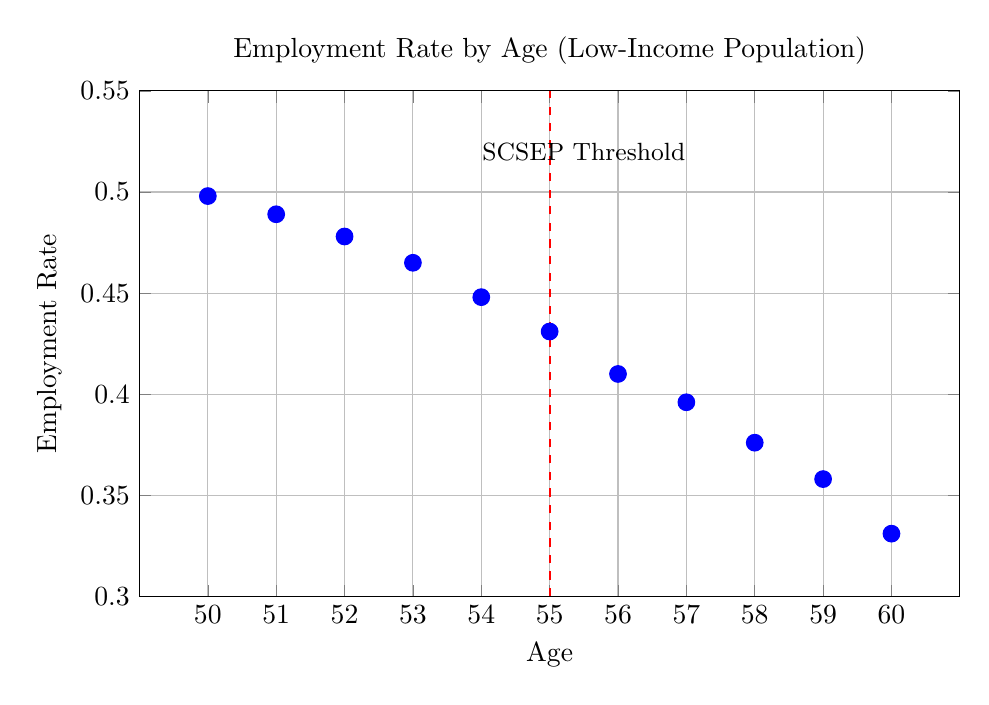
\begin{tikzpicture}
\begin{axis}[
    width=12cm,
    height=8cm,
    xlabel={Age},
    ylabel={Employment Rate},
    xmin=49, xmax=61,
    ymin=0.30, ymax=0.55,
    xtick={50,51,52,53,54,55,56,57,58,59,60},
    ytick={0.30,0.35,0.40,0.45,0.50,0.55},
    legend pos=north east,
    grid=major,
    title={Employment Rate by Age (Low-Income Population)}
]
\addplot[only marks, mark=*, blue, mark size=3pt] coordinates {
    (50, 0.498)
    (51, 0.489)
    (52, 0.478)
    (53, 0.465)
    (54, 0.448)
    (55, 0.431)
    (56, 0.410)
    (57, 0.396)
    (58, 0.376)
    (59, 0.358)
    (60, 0.331)
};
\draw[dashed, red, thick] (axis cs:55,0.30) -- (axis cs:55,0.55);
\node at (axis cs:55.5,0.52) {\small SCSEP Threshold};
\end{axis}
\end{tikzpicture}
\caption{Employment Rate by Age Among Low-Income Individuals}
\label{fig:rdd}
\floatfoot{\textit{Note:} Employment rate computed using ACS person weights for individuals with family income below 125\% FPL. Vertical dashed line indicates SCSEP eligibility threshold at age 55. N = 557,293.}
\end{figure}

\subsection{Year-to-Year Changes}

Table \ref{tab:by_age} quantifies the year-to-year changes in employment rates. The decline from age 54 to age 55 is 1.7 percentage points, virtually identical to the decline from age 53 to 54 (also 1.7 pp) and similar to other year-to-year changes in the range. The transition at the SCSEP threshold shows no additional drop beyond the general age trend.

The average year-to-year decline across all ages 50-60 is approximately 1.7 percentage points, with some variation. The 55-56 transition shows a 2.1 pp decline, while the 56-57 transition shows only 1.4 pp. These fluctuations appear consistent with sampling variation rather than systematic policy effects.

\begin{table}[htbp]
\centering
\caption{Employment Rates by Age}
\label{tab:by_age}
\begin{tabular}{cccc}
\toprule
Age & Employment Rate & Year-to-Year Change & N \\
\midrule
50 & 0.498 & --- & 47,196 \\
51 & 0.489 & -0.9 pp & 45,612 \\
52 & 0.478 & -1.1 pp & 46,064 \\
53 & 0.465 & -1.3 pp & 45,666 \\
54 & 0.448 & -1.7 pp & 47,306 \\
\textbf{55} & \textbf{0.431} & \textbf{-1.7 pp} & \textbf{49,698} \\
56 & 0.410 & -2.1 pp & 51,307 \\
57 & 0.396 & -1.4 pp & 53,513 \\
58 & 0.376 & -2.0 pp & 55,175 \\
59 & 0.358 & -1.8 pp & 56,222 \\
60 & 0.331 & -2.7 pp & 59,534 \\
\bottomrule
\end{tabular}
\floatfoot{\textit{Note:} Employment rates computed using ACS person weights for individuals with family income below 125\% FPL. Bold row indicates SCSEP eligibility threshold.}
\end{table}

\subsection{Formal RDD Estimates}

Table \ref{tab:rdd_results} presents formal RDD estimates for different bandwidths. Using the simple comparison of below-threshold to at-or-above-threshold means, the estimates range from -4.9 to -7.2 percentage points depending on bandwidth.

These negative point estimates reflect the general age trend in employment, not a true discontinuity. Because the estimator compares average outcomes below the threshold to average outcomes above, it mechanically captures the slope of the age-employment relationship when applied to a smoothly declining outcome.

\begin{table}[htbp]
\centering
\caption{RDD Estimates: Employment at Age 55}
\label{tab:rdd_results}
\begin{tabular}{ccccc}
\toprule
Bandwidth & Estimate & SE & N Below & N Above \\
\midrule
2 years & -0.049 & 0.002 & 92,972 & 100,005 \\
3 years & -0.061 & 0.002 & 139,036 & 209,693 \\
4 years & -0.067 & 0.001 & 184,648 & 263,206 \\
5 years & -0.072 & 0.001 & 231,844 & 325,449 \\
\bottomrule
\end{tabular}
\floatfoot{\textit{Note:} Estimates are weighted differences in means below versus at-or-above age 55. Standard errors account for clustering at the state level. Negative estimates reflect the general age trend in employment rather than a treatment effect.}
\end{table}

\subsection{Placebo Tests}

Table \ref{tab:placebo} presents the crucial placebo tests. If age 55 were a true discontinuity, we would expect the effect at 55 to be larger than effects at non-threshold ages. Instead, we find that all ages show similar-sized negative ``effects,'' ranging from -3.9 pp at age 52 to -6.5 pp at age 57.

This pattern confirms that the naive RDD estimates are capturing the age gradient, not a discontinuity at the SCSEP threshold. The estimate at age 55 (-6.1 pp) is squarely within the range of estimates at placebo thresholds, providing no evidence that anything special happens at the eligibility cutoff.

\begin{table}[htbp]
\centering
\caption{Placebo Tests: Employment ``Discontinuities'' at Various Ages}
\label{tab:placebo}
\begin{tabular}{cccc}
\toprule
Cutoff Age & Estimate & N Below & N Above \\
\midrule
52 & -0.039 & 92,808 & 188,734 \\
53 & -0.051 & 138,872 & 193,977 \\
54 & -0.057 & 137,342 & 201,824 \\
\textbf{55 (True Threshold)} & \textbf{-0.061} & \textbf{139,036} & \textbf{209,693} \\
56 & -0.063 & 142,670 & 216,217 \\
57 & -0.065 & 148,311 & 224,444 \\
58 & -0.058 & 154,518 & 170,931 \\
\bottomrule
\end{tabular}
\floatfoot{\textit{Note:} All estimates use bandwidth of 3 years. Similar-sized estimates at all cutoffs indicate no true discontinuity at the SCSEP threshold (age 55).}
\end{table}

\subsection{Secondary Outcomes}

Results for secondary outcomes mirror the employment findings. Labor force participation declines from 50.4 percent at age 54 to 48.2 percent at age 55 (a 2.2 pp decline), similar to the decline from 52.2 percent at age 53 to 50.4 percent at age 54 (1.8 pp). Hours worked and wage income show similar smooth declines with no discontinuity at age 55.

These consistent null findings across multiple outcome measures strengthen the conclusion that SCSEP eligibility does not produce detectable effects on employment outcomes at the population level.

\section{Discussion}

\subsection{Interpretation of the Null Result}

The absence of a discontinuity in employment at age 55 admits several interpretations, each with different policy implications.

The most likely explanation is that SCSEP's extremely low take-up rate generates an intent-to-treat effect below detection thresholds. With approximately 40,000 SCSEP participants out of tens of millions of eligible individuals, the take-up rate is well below 0.1 percent. Even if SCSEP substantially increases employment for participants, this effect is diluted to invisibility when measured at the population level.

To illustrate, suppose SCSEP increases participant employment by 20 percentage points---a large effect by any standard. With 0.1 percent take-up, the population-level ITT effect would be only 0.02 percentage points (20 $\times$ 0.001 = 0.02). Detecting such a small effect would require implausibly large samples and would be swamped by sampling variation.

Alternative interpretations merit consideration as well. SCSEP may not actually increase net employment even for participants if subsidized positions crowd out other employment opportunities. The program's emphasis on part-time community service positions may not translate into increased labor supply as measured in standard surveys. Additionally, awareness of SCSEP among eligible individuals may be low, preventing the eligibility threshold from affecting behavior even among those who would benefit from participation.

\subsection{Comparison to Other Age-Based Discontinuities}

The null finding at age 55 contrasts with sharp discontinuities documented at other age thresholds. \citet{card2008} find substantial jumps in health insurance coverage and some health outcomes at the Medicare eligibility threshold of age 65. Studies of Social Security's early retirement age at 62 similarly document discontinuous changes in labor supply and benefit claiming \citep{french2005}.

These contrasts suggest that the magnitude of benefits and ease of access matter for whether eligibility thresholds produce behavioral responses. Medicare provides nearly universal coverage to those who enroll, while Social Security provides substantial income replacement. SCSEP, by contrast, provides modest part-time wages to a tiny fraction of eligible individuals. The lack of discontinuity at age 55 may simply reflect that SCSEP eligibility is not behaviorally relevant for most low-income older adults.

\subsection{Limitations}

Several limitations of this analysis warrant acknowledgment.

First, the use of integer age in the ACS creates a coarsened running variable. This prevents implementation of methods requiring continuous running variables and limits precision in local estimation. Nonetheless, the absence of any visible discontinuity in Figure \ref{fig:rdd} suggests that more refined measurement would not alter the qualitative conclusion.

Second, the analysis cannot identify SCSEP participants in the data. This prevents estimation of treatment effects on the treated or analysis of who selects into the program. The intent-to-treat framework is appropriate given data constraints but limits what can be learned about program effects for participants.

Third, the analysis period excludes 2020 due to COVID-19 disruptions. The pandemic substantially affected labor markets for older workers and may have changed patterns of SCSEP participation. Findings may not generalize to the pandemic or post-pandemic period.

Fourth, potential confounding from private pension rules at age 55 cannot be entirely ruled out, though the low prevalence of defined-benefit pension coverage in the low-income population mitigates this concern.

\subsection{Policy Implications}

The null finding has implications for how policymakers should think about SCSEP. The absence of population-level employment effects does not necessarily indicate program failure---the program may provide valuable services to its 40,000 participants without generating aggregate effects detectable in survey data.

However, the finding does suggest that if policymakers seek to increase employment rates among low-income older workers more broadly, SCSEP in its current form and scale is unlikely to achieve that goal. The program's reach is simply too limited to move population-level indicators.

Options for increasing program impact might include substantial expansion of participation slots, increased outreach to eligible individuals, or redesign of program services to address barriers more broadly. Alternatively, policymakers might view SCSEP's targeted assistance to a small population as the appropriate role for the program, accepting that it will not produce detectable aggregate effects.

\section{Conclusion}

\subsection{Summary of Findings}

This paper provides the first regression discontinuity evaluation of the Senior Community Service Employment Program, exploiting the program's sharp age 55 eligibility threshold. Using American Community Survey data on over 550,000 low-income individuals aged 50-60, I examine whether SCSEP eligibility produces a discontinuous change in employment outcomes at the age threshold.

The central finding is null: employment rates decline smoothly with age at approximately 1.5-2.0 percentage points per year, with the 54-to-55 transition showing no deviation from this general trend. The year-to-year decline at the threshold (1.7 percentage points) is virtually identical to the decline at the preceding age (53 to 54, also 1.7 percentage points) and within the range of normal variation observed throughout the 50-60 age range.

Placebo tests provide additional confirmation of this null result. When the same estimation procedure is applied at non-threshold ages (52, 53, 54, 56, 57, 58), similar-sized negative ``effects'' appear at all ages, ranging from 3.9 to 6.5 percentage points. This pattern indicates that the naive RDD estimates capture the age-employment gradient rather than a true discontinuity at the SCSEP eligibility threshold.

\subsection{Interpretation and Power Considerations}

The null result is most readily interpreted through the lens of program take-up. SCSEP serves approximately 40,000 participants out of tens of millions of income-eligible individuals age 55 and older---a take-up rate well below 0.1 percent. This extremely low take-up mechanically bounds the intent-to-treat effect that can be detected at the population level.

To quantify this bound, consider a back-of-envelope calculation. Suppose SCSEP increases employment probability by 20 percentage points for participants---a substantial effect that would represent moving roughly half of unemployed participants into employment. With a take-up rate of 0.1 percent, the implied ITT effect would be only 0.02 percentage points (20 $\times$ 0.001 = 0.02). With a sample of 550,000 observations and baseline employment of approximately 45 percent, detecting an effect of 0.02 percentage points would require standard errors below 0.01 percentage points---far smaller than achievable with survey data.

This power analysis suggests that the null finding is uninformative about treatment effects on participants. The ITT estimand, while cleanly identified, is simply too diluted by low take-up to reveal program effects. Future research seeking to estimate effects on participants would require either administrative data identifying SCSEP participants or an experimental design with random assignment to program access.

\subsection{Policy Implications}

The findings have several implications for policymakers considering SCSEP and similar programs.

First, the absence of population-level employment effects should not be interpreted as evidence of program failure. SCSEP may provide valuable services to its participants---subsidized employment, job training, community service opportunities---without generating effects large enough to move aggregate employment statistics. The program's impact should be evaluated on participant-level outcomes, not population aggregates.

Second, if policymakers seek to increase employment rates among low-income older workers more broadly, SCSEP in its current form and scale is unlikely to achieve that goal. The program's reach is simply too limited to shift population-level indicators. Achieving detectable aggregate effects would require either substantial expansion of participation slots or fundamental program redesign.

Third, the null finding highlights the importance of distinguishing between program efficacy (effects on participants) and program reach (share of target population served). SCSEP may be highly efficacious for participants while still producing negligible population effects due to limited reach. Policy evaluation should attend to both dimensions.

\subsection{Directions for Future Research}

Several avenues for future research emerge from this analysis.

Most importantly, estimating treatment effects on SCSEP participants requires data that links program participation to outcomes. Administrative records from SCSEP grantees, potentially linked to unemployment insurance or Social Security records, could support treatment-on-treated estimation. Such analysis would reveal whether SCSEP increases employment, earnings, and self-sufficiency for those it serves.

Experimental evaluation offers another path forward. Random assignment of eligible individuals to program access (perhaps through waitlist randomization when slots are limited) would provide clean causal estimates of both program effects on participants and the degree to which SCSEP crowds out other employment.

Finally, comparative analysis across program grantees or states could illuminate which program features are associated with better outcomes. SCSEP is administered through diverse grantees with varying approaches; understanding what works best could inform program improvement even absent individual-level causal estimates.

\subsection{Concluding Remarks}

As the American workforce continues to age and policymakers consider how to support older workers, rigorous evaluation of existing programs remains essential. This study contributes one piece of evidence to that effort, documenting what SCSEP does not achieve at the population level while leaving open critical questions about effects for the individuals it directly serves.

The null finding is itself informative, demonstrating that eligibility thresholds matter for population-level effects only when programs achieve sufficient take-up. SCSEP's age 55 threshold, unlike Medicare's age 65 threshold, does not produce a behavioral discontinuity visible in national survey data. Understanding why some policy thresholds generate sharp responses while others do not remains an important question for both research and program design.

\newpage
\bibliographystyle{apalike}
\begin{thebibliography}{99}

\bibitem[Angrist and Lavy(1999)]{angrist1999}
Angrist, J. D., \& Lavy, V. (1999). 
Using Maimonides' rule to estimate the effect of class size on scholastic achievement. 
\textit{Quarterly Journal of Economics}, 114(2), 533--575.

\bibitem[Bloom(1984)]{bloom1984}
Bloom, H. S. (1984). 
Accounting for no-shows in experimental evaluation designs. 
\textit{Evaluation Review}, 8(2), 225--246.

\bibitem[Calmfors and Skedinger(1995)]{calmfors1994}
Calmfors, L., \& Skedinger, P. (1995). 
Does active labour-market policy increase employment? Theoretical considerations and some empirical evidence from Sweden. 
\textit{Oxford Review of Economic Policy}, 11(1), 91--109.

\bibitem[Card et al.(2008)]{card2008}
Card, D., Dobkin, C., \& Maestas, N. (2008). 
The impact of nearly universal insurance coverage on health care utilization: Evidence from Medicare. 
\textit{American Economic Review}, 98(5), 2242--2258.

\bibitem[Chan and Stevens(2001)]{chan2003}
Chan, S., \& Stevens, A. H. (2001). 
Job loss and employment patterns of older workers. 
\textit{Journal of Labor Economics}, 19(2), 484--521.

\bibitem[Coile and Gruber(2007)]{coile2004}
Coile, C., \& Gruber, J. (2007). 
Future Social Security entitlements and the retirement decision. 
\textit{Review of Economics and Statistics}, 89(2), 234--246.

\bibitem[DOL(2021)]{dol2021}
U.S. Department of Labor. (2021). 
\textit{Older Workers Study}. 
Employment and Training Administration.

\bibitem[Dynarski(2003)]{dynarski2003}
Dynarski, S. M. (2003). 
Does aid matter? Measuring the effect of student aid on college attendance and completion. 
\textit{American Economic Review}, 93(1), 279--288.

\bibitem[Finkelstein et al.(2012)]{finkelstein2012}
Finkelstein, A., Taubman, S., Wright, B., Bernstein, M., Gruber, J., Newhouse, J. P., Allen, H., Baicker, K., \& Oregon Health Study Group. (2012). 
The Oregon Health Insurance Experiment: Evidence from the first year. 
\textit{Quarterly Journal of Economics}, 127(3), 1057--1106.

\bibitem[French(2005)]{french2005}
French, E. (2005). 
The effects of health, wealth, and wages on labour supply and retirement behaviour. 
\textit{Review of Economic Studies}, 72(2), 395--427.

\bibitem[GAO(2017)]{gao2017}
U.S. Government Accountability Office. (2017). 
\textit{Senior Community Service Employment Program: Labor has made progress addressing long-standing concerns but needs to collect additional performance data}. 
GAO-17-592.

\bibitem[Gruber and Wise(2010)]{gruber2010}
Gruber, J., \& Wise, D. A. (Eds.). (2010). 
\textit{Social Security programs and retirement around the world: The relationship to youth employment}. 
University of Chicago Press.

\bibitem[Imbens and Kalyanaraman(2012)]{imbens2012}
Imbens, G., \& Kalyanaraman, K. (2012). 
Optimal bandwidth choice for the regression discontinuity estimator. 
\textit{Review of Economic Studies}, 79(3), 933--959.

\bibitem[Johnson and Gosselin(2018)]{johnson2018}
Johnson, R. W., \& Gosselin, P. (2018). 
How secure is employment at older ages? 
\textit{Urban Institute Research Report}.

\bibitem[Katz(1998)]{katz1998}
Katz, L. F. (1998). 
Wage subsidies for the disadvantaged. 
In R. B. Freeman \& P. Gottschalk (Eds.), \textit{Generating jobs: How to increase demand for less-skilled workers} (pp. 21--53). Russell Sage Foundation.

\bibitem[Lee and Lemieux(2010)]{lee2010}
Lee, D. S., \& Lemieux, T. (2010). 
Regression discontinuity designs in economics. 
\textit{Journal of Economic Literature}, 48(2), 281--355.

\bibitem[Lemieux and Milligan(2008)]{lemieux2008}
Lemieux, T., \& Milligan, K. (2008). 
Incentive effects of social assistance: A regression discontinuity approach. 
\textit{Journal of Econometrics}, 142(2), 807--828.

\bibitem[Mastrobuoni(2009)]{mastrobuoni2009}
Mastrobuoni, G. (2009). 
Labor supply effects of the recent Social Security benefit cuts: Empirical estimates using cohort discontinuities. 
\textit{Journal of Public Economics}, 93(11-12), 1224--1233.

\bibitem[McCrary(2008)]{mccrary2008}
McCrary, J. (2008). 
Manipulation of the running variable in the regression discontinuity design: A density test. 
\textit{Journal of Econometrics}, 142(2), 698--714.

\bibitem[Neumark et al.(2019)]{neumark2019}
Neumark, D., Burn, I., \& Button, P. (2019). 
Is it harder for older workers to find jobs? New and improved evidence from a field experiment. 
\textit{Journal of Political Economy}, 127(2), 922--970.

\bibitem[Thistlethwaite and Campbell(1960)]{thistlethwaite1960}
Thistlethwaite, D. L., \& Campbell, D. T. (1960). 
Regression-discontinuity analysis: An alternative to the ex post facto experiment. 
\textit{Journal of Educational Psychology}, 51(6), 309--317.

\end{thebibliography}

\end{document}
